
\section{Measurement invariance in categorical data}
\label{sec:invariance}
\subsection{The problem of measurement invariance}

Many important variables in the social sciences are not or cannot be directly observed, but are instead latent  \citep{bollen2002latent} and measured using a vector of multiple indicators, $\mathbf{y}$, say. This measurement of the latent variable $x$ is defined by a ``measurement model'',
\begin{equation}
	p(\mathbf{y} | x).
		\label{eq:measurement-model}
\end{equation}
The latent $x$ variable could, for example, be a ``random effect'', a person's unobserved utility for a choice, a general attitude, or a variable measured with error such as voter turnout.
Often the measurement model in Equation \ref{eq:measurement-model} is not, however, of primary interest to the researcher, but rather  the relationship between the latent variable and some covariate vector $\mathbf{z}$ is, i.e. the ``structural model'',
\begin{equation} 
	p(x | \mathbf{z}).
		\label{eq:structural-model}
\end{equation}
Figure \ref{fig:LVM} shows this relationship as an arrow between the observed covariate $\mathbf{z}$ and latent variable $x$.
For example, $\mathbf{z}$ could contain a set of dummy variables indicating a respondent's country or gender, so that Equation \ref{eq:structural-model} simply compares values of $x$ across countries or genders. Alternatively, interest could focus on the influence of continuous covariates such as GDP or age on the latent $x$. Of course, the problem is that $x$ is not observed, but only $\mathbf{y}$ and $\mathbf{z}$ are. 

\begin{figure}\centering
	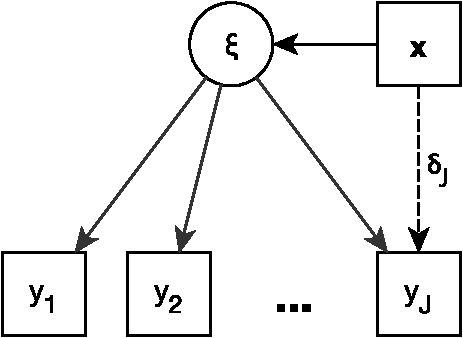
\includegraphics[width=.4\textwidth]{figures/LVM}
	\caption{Graph of a latent variable model. The latent variable $x$ is shown in a circle to indicate that it is unobserved. }
	\label{fig:LVM}
\end{figure}

Latent variable models generally attack this problem by making two key assumptions about how $x$ is measured \citep{skrondal2004generalized}. The first assumption is necessary to identify the measurement model. It states that, given the latent variable, the indicators $y_j$ are ``locally independent'': $
%\begin{equation}
		p(\mathbf{y} | x) = \prod_{j \in \{1..J\}} p(y_j | x),
%		\label{eq:local-independence}
%\end{equation} 
$ where $J$ is the number of indicators use to measure $x$; typically $J$ will be at least three. In Figure \ref{fig:LVM}, the  absence of relationships among the observed variables except those due to their common cause $x$ implies local independence.
%The local independence assumption is common to all multiple indicator latent variable models and not specific to the issue of relating the covariate to the latent variable. 

The second assumption is necessary to identify the structural model. It states that, while the latent variable may depend on the covariate, its \emph{measurement} should not, i.e. the indictors should be ``measurement invariant'':
\begin{equation}
	p(y_j | x, \mathbf{z}) = p(y_j | x).
	\label{eq:no-dif}
\end{equation}
When Equation \ref{eq:no-dif} holds for \emph{all} $J$ indicators this is called ``full measurement invariance'' \citep{meredith1993measurement}. 
A violation of  measurement invariance is sometimes termed ``differential item functioning'' (DIF), since the ``items'' $y_j$ have differing conditional probability distributions given $x$ for differing values of $\mathbf{z}$ \citep{mellenbergh1989item}.
Intuitively, measurement invariance is necessary to identify the structural model of Equation \ref{eq:structural-model} because if all indicators are caused by both $x$ and $\mathbf{z}$, then there is no way of knowing whether an observed indicator difference  over values of the covariate is due to a covariate effect on  $x$ or to a difference over the covariate in the way $x$ is measured. For example, when comparing countries, an observed cross-country difference in anti-immigrant attitudes might be a substantive difference or it might equally well be explained as differing answer tendencies over countries. 
%Since the same is true for all the other indicators, there is just no way of separating effects on indicators from effects on the latent variable: the structural model is therefore unidentifiable.  Full measurement invariance thus guarantees that $x$ can indeed be compared across values of the covariates.

This identification problem only occurs, however, when there are no measurement invariant indicators at all. A single invariant indicator can disentangle measurement from substantive differences in the other, non-invariant, indicators. Full measurement invariance is therefore not necessary to identify the structural model, but ``partial measurement invariance'' is \citep{byrne1989testing}. The standard practice is to search for non-invariant indicators and either remove them or parameterize their differential functioning \citep{Holland:1993aa}. 
A common way of doing so when the observed variables are categorical with $K$ categories is a logistic regression, 
\begin{equation}
	P(Y_j = k) = \frac{\exp(\tau_{jk} + \lambda_{jk} x + \delta_{jk} \mathbf{z})}{\sum_{m \in \{1..K\}} \exp(\tau_{jm} + \lambda_{jm} x + \delta_{jm} \mathbf{z})},
	\label{eq:logistic-dif}
\end{equation}
\citep{mellenbergh1989item,kankaras2010testing}, where some restriction is imposed on the parameters for identification purposes such as ``effect coding'', $\sum_k \tau_{jk} = \sum_k \lambda_{jk} =\sum_k \delta_{jk} = 0$, or dummy coding, $\tau_{j1} = \lambda_{j1} = \delta_{j1} = 0$. 
It can be seen in Equation \ref{eq:logistic-dif} that setting $\delta_{jk} = 0$ corresponds to measurement invariance\footnote{An interaction term $\delta_{jk}^* \mathbf{z}x$ could be added to Equation \ref{eq:logistic-dif} but has been omitted for clarity.}. This means that it is possible to estimate a model in which $\delta_{jk} \neq 0$ for \emph{some} indicators, while $\delta_{jk}$ is kept at zero, i.e. partially measurement invariant, for others. 
Figure \ref{fig:LVM} shows this possible direct effect from covariate to indicator as a dashed arrow. 

\subsection{Existing solutions}

In short, some form of measurement invariance is needed to estimate the structural model of interest: deciding which form, that is, selecting a model, is therefore crucial. Currently, there are broadly three existing approaches to doing so:
\begin{enumerate}
	\item Selecting one indicator as the reference indicator or ``anchor item'' \emph{a priori};
	\item Imposing a strong prior on the differential functioning parameters \citep{muthen2012bayesian};
	\item Testing the null hypothesis of full measurement invariance \citep{steenkamp_assessing_1998,french2006confirmatory} or partial measurement invariance, in which violations of invariance are freed  \citep{byrne1989testing,saris2009testing}.
\end{enumerate}

\emph{A priori} reference indicators are often selected implicitly, for example by setting one loading to unity in multiple group CFA. A recent extension to this approach, the ``alignment method'', was suggested by \citet{muthen2014alignment}. When the researcher is not certain that the ``reference indicator'' is indeed invariant, however, it is impossible to select it based on the data \citep{hancock2009tenuousness}. The Bayesian approach suggested by \citet{muthen2012bayesian} has the distinct advantage that, when the prior has been chosen aptly, the data can determine which indicators should be more or less invariant -- hence the term ``approximate measurement invariance'' \citep[see also][]{schoot2013facing}. However, if the prior is not chosen adequately, for instance if it is too strong or too weak, bias in the parameters of interest may still occur. At current this remains a topic for future study, although the approach is promising. Finally, it is common to test for full or partial measurement invariance using various fit measures available for this purpose \citep{byrne1989testing,hu1998fit,cheung2002evaluating,chen2007sensitivity,saris2009testing}. However, this approach has recently been shown to have an unfortunate disadvantage: when a violation is detected, it need not have seriously affected the parameter of interest, and when an invariance model is selected, substantial bias in the parameter of interest may still remain \citep{Oberski:WP:EPC-interest}. In short, while measurement invariance is an important assumption in latent variable modeling, the existing methods do not directly account for the effect that violations of this assumption have on the parameters of interest.

To complement measurement invariance testing, the 
 EPC-interest was therefore recently introduced by \citet{Oberski:WP:EPC-interest} for continuous data structural equation models. The EPC-interest assesses what would happen if a particular possible direct effect were freed. Rather than assessing the size of this direct effect itself, however, it assesses its impact on the parameter of interest. However, this measure is only available for continuous data, whereas many important measures of latent variables in the social sciences are categorical. Examples include the votes (Yea/Nay) of senators indicating their ideology, how respondents rank their value priorities (1 through 4), or answers (correct/incorrect) to political knowledge questions. The following section therefore extends the EPC-interest to the case of categorical indicators.

\subsection{EPC-interest}
\label{sec:epc-interest}

The ``$\da$'' estimates the change in a free parameter estimate of the model that one can expect to observe if a particular restriction were freed. It is therefore a method of sensitivity analysis. However, the researcher is not forced to estimate all possible alternative models, but can evaluate the sensitivity of the results after fitting the restrictive full invariance model. 
The $\da{}$ is based on the work of \citet{saris_detection_1987}, who introduced the expected parameter change in a fixed parameter for linear structural equation models (SEM), and \citet{bentler1993some}, who introduced the expected parameter change in a free parameter after freeing a fixed parameter for SEM. It was applied to invariance testing with continuous data by \citet{Oberski:WP:EPC-interest}.

In models for categorical data, the EPC-interest can be derived, as shown below and in the Appendix, by applying general results of maximum likelihood analysis. An additional problem with categorical data, however, is that there are usually sets of parameters relating to particular variables. For example, in Equation \ref{eq:logistic-dif}, there will be $K$ ``loadings'' $\lambda_{jk}$, $K$ ``intercepts'' $\tau_{jk}$,  $K$ ``direct effects'' $\delta_{jk}$, and, if present, $K$ ``interaction effects'' $\delta^*_{jk}$ for each variable. This principle may be familiar from ANOVA: when an ANOVA term corresponds to a categorical variable, it will have several parameters that are considered simultaneously in the analysis. These parameters will, moreover, be strongly dependent on one another, so that the impact of freeing one of them cannot be seen separately from the impact of freeing another parameter relating to the same variable. 

For this reason, when extending EPC-interest to the categorical case, it also becomes necessary to allow for the consideration of \emph{sets} of parameters to free rather than just investigating the effect of single restrictions. This requires a multivariate EPC-interest, rather than the univariate one in use so far. Furthermore, while for linear SEM estimates the necessary closed-form expected gradients and hessians are available \citep{Oberski:WP:EPC-interest}, in order to extend the EPC-interest to categorical data models, which differ considerably in the form these quantities take, we will take a more general approach here.

%For example, in structural equation models with ordered categorical indicators \citep{muthen_general_1984}, we would recommend considering the effect of freeing all thresholds as a set, rather than considering the effect of the threshold for each category separately. By the model's definition, such parameters are strongly dependent. 

In deriving the EPC-interest, the key concept is considering the likelihood not only as a function of the free parameters of the model, but also as a function of the parameters that are fixed to obtain the full invariance model. Collecting the free parameters in a vector $\param$ and the fixed parameters in a vector $\bpsi$, we assume the likelihood can be written as an explicit function of both sets of parameters, $L(\param, \bpsi)$.  The maximum-likelihood estimates $\that$ of the free parameters can then be seen as obtained under the full invariance model that sets $\bpsi=0$, i.e. $\that = \arg\max_{\param} L(\param, \bpsi = 0)$. Further, define the parameters of substantive interest as $\vm{\pi} := \vm{P} \param$, where $\vm{P}$ is typically a logical (0/1) selection matrix, although any linear function of the free parameters $\param$ may be taken. 
Interest then focuses on the likely value these free parameters $\vm{\pi}$ would take if the fixed $\bpsi$ parameters were freed in an alternative model, $\hat{\vm{\pi}}_a = \vm{P} \arg\max_{\param, \bpsi} L(\param, \bpsi)$. 

We now show how these changes in the parameters of interest as a consequence of freeing the fixed parameters $\bpsi$ can be estimated without fitting the alternative model. Let the Hessian $\hat{\vm{H}}_{\vm{a}\vm{b}}$ be the matrix of second derivatives of the likelihood with respect to vectors $\vm{a}$ and $\vm{b}$, evaluated at the maximum likelihood solution of the full invariance model, $\hat{\vm{H}}_{\vm{a}\vm{b}} := (\partial^2 L /\partial \vm{a} \partial \vm{b}^\prime)|_{\param=\that}$. 
The expected change in the parameters of interest is then measured by the $\da$, 
\begin{equation}
\da = \hat{\vm{\pi}}_a - \hat{\vm{\pi}} = \vm{P}
%	\left( \frac{\partial^2 L(\param, \bpsi)}{\partial (\param, \bpsi)^\prime \partial (\param, \bpsi)} \right)^{-1}
%		\vm{D}^{-1} \hat{\vm{H}}_{\param\bpsi}^\prime \hat{\vm{H}}^{-1}_{\param\param}
\hat{\vm{H}}^{-1}_{\param\param} \hat{\vm{H}}_{\param\bpsi}\vm{D}^{-1}
		\left[ \left.\frac{\partial L(\param, \bpsi)}{\partial \bpsi}\right|_{\param = \that} \right] +	
		O(\vm{\delta}^\prime\vm{\delta}),
		\label{eq:epc-interest}
\end{equation}
where $\vm{D}:= \hat{\vm{H}}_{\bpsi\bpsi} - \hat{\vm{H}}_{\param\bpsi}^\prime \hat{\vm{H}}^{-1}_{\param\param} \hat{\vm{H}}_{\param\bpsi}$ and the deviation from the true values is $\vm{\delta}:= \vm{\vartheta} - \hat{\vm{\vartheta}}$, with $\vm{\vartheta}$ collecting the free and fixed parameters in a vector, $\vm{\vartheta}:= (\param^\prime, \bpsi^\prime)^\prime$. Note that, apart from the order of approximation term $O(\vm{\delta}^\prime \vm{\delta})$,  Equation \ref{eq:epc-interest} contains only terms that can be calculated after fitting the invariance model.
%(Relevant derivatives for the special case of the multilevel latent class model are given in Appendix \ref{app:derivatives}.)
 Thus, it is not necessary to fit the alternative model to obtain the $\da{}$.

In the structural equation modeling literature, the expected change in the fixed parameters $\bpsi$  is commonly found and implemented in standard SEM software. This measure is commonly know as the ``EPC'', but to avoid confusion we term it ``EPC-self'' here. The EPC-self and $\da{}$ both consider the impact of freeing restrictions, but differ in the target of this impact: the EPC-self evaluates the impact on the restriction itself, whereas the $\da{}$ evaluates the impact on the parameters of interest. In spite of these differences, the two measures are related: this can be seen by recognizing that $- \vm{D}^{-1}
		\left[ \left.\frac{\partial L(\param, \bpsi)}{\partial \bpsi}\right|_{\param = \that} \right] = \text{EPC-self} \approx \bpsi - \hat{\bpsi}$ so that, from Equation \ref{eq:epc-interest}, 
\begin{equation}
\da=- \vm{P} \hat{\vm{H}}^{-1}_{\param\param} \hat{\vm{H}}_{\param\bpsi} \,\text{EPC-self} \approx
- \vm{P} \hat{\vm{H}}^{-1}_{\param\param} \hat{\vm{H}}_{\param\bpsi} \left( \bpsi - \hat{\bpsi}\right)
\end{equation}
Furthermore, since $\hat{\bpsi}$ and $\hat{\param}$ are implicitly related by the fact that they are both solutions to the equation $\partial L / \partial \vm\vartheta = \vm{0}$, invoking the implicit function theorem yields $- \hat{\vm{H}}^{-1}_{\param\param} \hat{\vm{H}}_{\param\bpsi}  = \partial \param / \partial \bpsi^\prime$, so that 
\begin{equation}
	\da = \vm{P} \left( \frac{\partial \param} {\partial \bpsi^\prime} \right) \left( \bpsi - \hat{\bpsi}\right),
	\label{eq:epc-linear}
\end{equation}
that is, the $\da{}$ can be seen simply as the coefficient of a linear approximation to the relationship between the free and fixed parameters, multiplied by the change in the fixed parameters. This demonstrates the difference with the sensitivity analysis approach common in econometrics \citep[p. 168]{magnus2007local} in which only $\partial \param / \partial \bpsi^\prime$ is considered: the $\da{}$ combines both the direction ($\partial \param / \partial \bpsi^\prime$) and the magnitude ($ \bpsi - \hat{\bpsi}$) of the misspecification.


The accuracy of the approximation of the $\da{}$ as a measure of the change in the parameters of interest is reflected in the order of approximation term, $O(\vm{\delta}^\prime\vm{\delta})$. It can be seen that this accuracy is quadratic in the overall change in parameters, so that the approximation can be expected to work best when the misspecifications are not ``too large''. This result corresponds to results on the score test (``modification index'') and ``EPC-self'' in the literature on structural equation modeling, which can be shown to be exact under a ``sequence of local alternatives'', i.e. when $\vm{\vartheta} = \lim_{n\rightarrow\infty} \hat{\vm{\vartheta}} + n^{-\frac{1}{2}}\vm{\delta}$ \citep[p. 135]{satorra1989alternative}.
It is important to note here that $\vm{\delta}$ is the deviation from the ``true'' value of $\vm{\vartheta}$, rather than the deviation from the limit of the parameter estimates under the alternative model. Therefore another view on the accuracy is that it will be better when the alternative model is not strongly misspecified. For this reason it is also important to consider freeing sets of very strongly related parameters simultaneously, since a change in one of them will then imply a change in the others, and, consequently, a misspecified alternative model.

